\documentclass[tikz,border=5]{standalone}
\usetikzlibrary{graphs,arrows.meta,arrows, positioning, automata}

\begin{document}

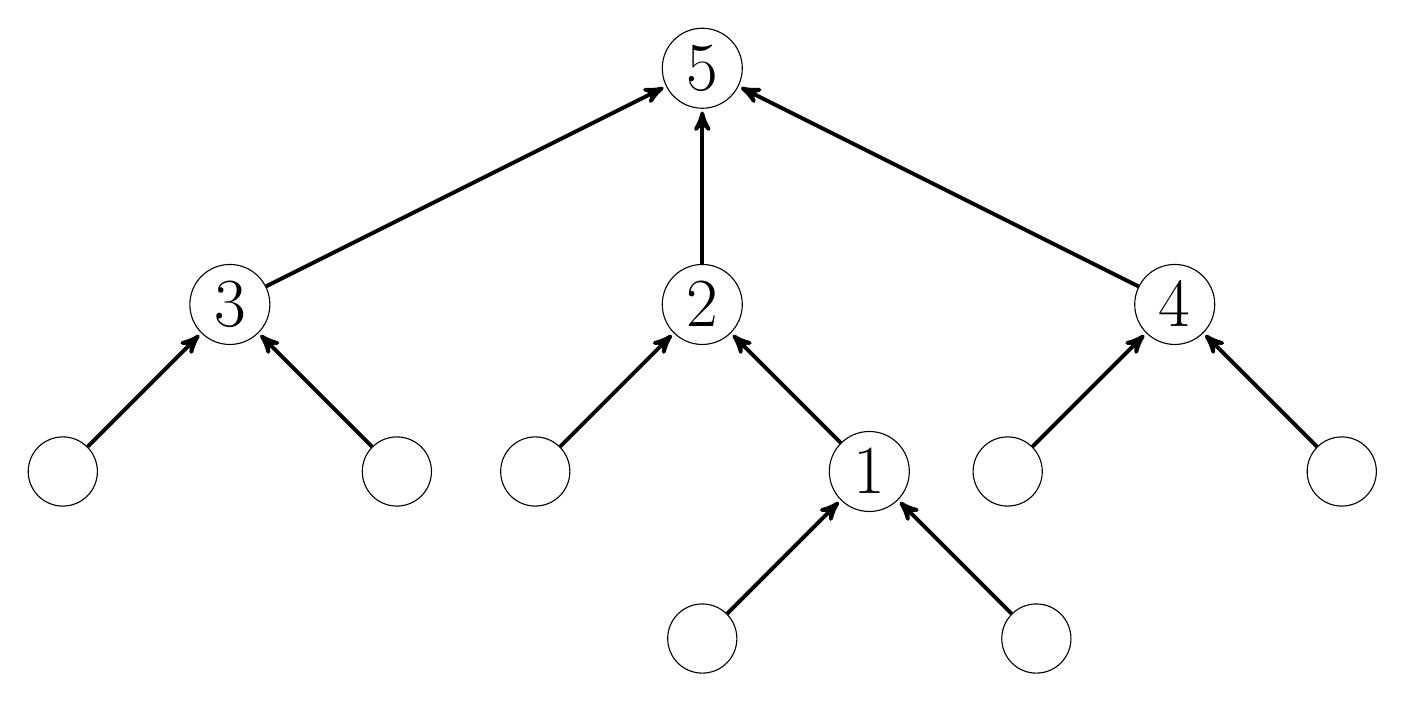
\begin{tikzpicture}[>=stealth',shorten >=1pt,node distance=3cm,on grid,initial/.style={}]
    \node[state] (T5) at (0,0) {\Huge $5$};
    \node[state] (T2) at (0,-3) {\Huge $2$};
    \node[state] (T3) at (-6,-3) {\Huge $3$};
    \node[state] (T4) at (6,-3) {\Huge $4$};
    \node[state] (T3_C1) [below left =of T3] {};
    \node[state] (T3_C2) [below right =of T3] {};
    \node[state] (T2_C1) [below left =of T2] {};
    \node[state] (T1) [below right =of T2] {\Huge $1$};
    \node[state] (T4_C1) [below left =of T4] {};
    \node[state] (T4_C2) [below right =of T4] {};
    \node[state] (T1_C1) [below left =of T1] {};
    \node[state] (T1_C2) [below right =of T1] {};

    \tikzset{mystyle/.style={->,double=black}}
    %\tikzset{every node/.style={fill=white}}
    \path (T3) edge [mystyle] node {} (T5);
    \path (T2) edge [mystyle] node {} (T5);
    \path (T4) edge [mystyle] node {}  (T5);
    \path (T3_C1) edge [mystyle] node {} (T3);
    \path (T3_C2) edge [mystyle] node {} (T3);
    \path (T2_C1) edge [mystyle] node[pos=0.5] {} (T2);
    \path (T1) edge [mystyle] node {} (T2);
    \path (T4_C1) edge [mystyle] node {} (T4);
    \path (T4_C2) edge [mystyle] node {} (T4);
    \path (T1_C1) edge [mystyle] node {} (T1);
    \path (T1_C2) edge [mystyle] node {} (T1);
\end{tikzpicture}

\end{document}